\documentclass[addpoints,10pt]{exam}

\usepackage{amsmath,amsthm,enumitem,wrapfig,amsfonts,mathtools}
\usepackage[mathscr]{euscript}
\usepackage[super]{nth}
\usepackage{dsfont}
\usepackage{xparse}
\usepackage{cancel}

\usepackage{geometry}
\usepackage[T1]{fontenc} % Use 8-bit encoding that has 256 glyphs
\renewcommand{\rmdefault}{ptm} %Change the Front Family from the default(cmr) to ptm(Times)
\usepackage{amsmath,amsfonts,amsthm,amssymb} % Math packages
\usepackage{bm}
%\usepackage{mathptmx}
\usepackage{graphicx}
\usepackage{sectsty} % Allows customizing section commands
% \allsectionsfont{\centering} % Make all sections centered, the default font and small caps

\usepackage{pgfplots}
\pgfplotsset{compat=1.18}
\usetikzlibrary{arrows.meta}
\usepackage{xcolor}
\definecolor{darkpastelgreen}{rgb}{0.01, 0.75, 0.24}
\definecolor{blue-violet}{rgb}{0.54, 0.17, 0.89}
%\usepackage{polylongdiv} %polynomial long division
% Custom problem environmenturther
\usepackage{polynom}
\newcounter{cprob}
\newenvironment{cprob}[1]{%
    \setcounter{cprob}{#1}%
    \noindent\textbf{Problem \thecprob.}%
}{%
    \par\bigskip%
}

\usepackage{ytableau} %young tableau

\theoremstyle{plain}
\newcommand{\theoremname}{Theorem}
\newtheorem{thm}{\protect\theoremname}
  \theoremstyle{definition}
  \newtheorem{prob}[thm]{Problem}
  \newtheorem*{problem*}{Open Problem}
  \theoremstyle{plain}
  \newtheorem{conjecture}[thm]{Conjecture}
  \theoremstyle{plain}
  \newtheorem{lem}[thm]{Lemma}
  \newtheorem*{lem*}{Lemma}
  \newtheorem{obs}[thm]{Observation}
  \newtheorem{cor}[thm]{Corollary}
  \theoremstyle{definition}
\newtheorem{definition}[thm]{Definition}
\newcommand{\subsetdot}{\mathrel{\subset\mkern-13mu\cdot\mkern4mu}}




% Patch prob environment to be single spaced
\let\oldprob\prob
\let\endoldprob\endprob
\renewenvironment{prob}
  {\begin{singlespace}\oldprob}
  {\endoldprob\end{singlespace}}

% start problem one line below like for enumerated problems with multiple parts
\newcommand{\belowtitle}{\leavevmode\newline}
%\Observe command
\newcommand{\Observe}{\text{Observe.}}
%(=>)
\newcommand{\IF}{\mathbf{(\Rightarrow)}}
%(<=)
\newcommand{\FI}{\mathbf{(\Leftarrow)}}
%equivalence classes; \class[S]{ *content in square brackets* }
\newcommand{\class}[2][]{\ensuremath{\left[\,#2\,\right]_{#1}}}

\newcommand{\horrule}[1]{\rule{\linewidth}{#1}}
\newcommand{\kkk}{\ensuremath{\Bbbk}} 
\newcommand{\CC}{\ensuremath{\mathbb{C}}}
\newcommand{\FF}{\ensuremath{\mathbb{F}}}
\newcommand{\KK}{\ensuremath{\mathbb{K}}}
\newcommand{\NN}{\ensuremath{\mathbb{N}}}
\newcommand{\QQ}{\ensuremath{\mathbb{Q}}} 
\newcommand{\RR}{\ensuremath{\mathbb{R}}} 
\newcommand{\ZZ}{\ensuremath{\mathbb{Z}}}
\newcommand{\MM}{\ensuremath{\mathcal{M}}}
\newcommand{\TT}{\ensuremath{\mathcal{T}}}
\newcommand{\BB}{\ensuremath{\mathcal{B}}}
\newcommand{\VV}{\ensuremath{\mathcal{V}}}
\newcommand{\WW}{\ensuremath{\mathcal{W}}}
\newcommand{\UU}{\ensuremath{\mathcal{U}}}
\newcommand{\PP}{\ensuremath{\mathcal{P}}}
\newcommand{\LL}{\ensuremath{\mathcal{L}}}
\newcommand{\kk}{\ensuremath{\mathds{k}}}
\newcommand{\EE}{\ensuremath{\mathbb{E}}}
\newcommand{\A}{\ensuremath{\mathcal{A}}}
\newcommand{\YY}{\ensuremath{\mathcal{Y}}}



\newcommand{\sm}{\char`\\}
%vector stuff
\DeclarePairedDelimiter{\ip}{\langle}{\rangle} %inner product/generate
\DeclarePairedDelimiter{\norm}{\lVert}{\rVert} %norm
\DeclarePairedDelimiter{\sqb}{\lbrack}{\rbrack} %corrd

\newcommand{\floor}[1]{\left\lfloor #1 \right\rfloor}
\newcommand{\ceil}[1]{\left\lceil #1 \right\rceil}
\newcommand{\mbf}[1]{\ensuremath{\mathbf{#1}}}
\newcommand{\tbf}[1]{\textbf{ #1 }}
\newcommand{\Span}{\ensuremath{\mathrm{Span}}}
\newcommand{\Char}[1]{\mathrm{Char}\; #1}
\DeclareMathOperator{\lcm}{lcm}
\newcommand{\id}{\ensuremath{\mathrm{id}}}
\newcommand{\Gal}[2]{\mathrm{Gal}(#1/#2)}
\newcommand{\Aut}{\ensuremath{\mathrm{Aut}}}
\newcommand{\Fix}[2]{\mathrm{Fix}_{#1}(#2)}
\newcommand{\nil}{\ensuremath{\mathrm{nil}}}
\newcommand{\Hom}{\ensuremath{\mathrm{Hom}}}
\newcommand{\Obj}{\ensuremath{\mathrm{Obj}}}

\newcommand{\Rng}{\ensuremath{\mathrm{Rng}}}
\newcommand{\Ring}{\ensuremath{\mathrm{Ring}}}

\newcommand{\Rect}{\ensuremath{\operatorname{Rect}}}





\makeatletter
\renewcommand*\env@matrix[1][*\c@MaxMatrixCols c]{%
  \hskip -\arraycolsep
  \let\@ifnextchar\new@ifnextchar
  \array{#1}}
\makeatother

\def\env@matrix{\hskip -\arraycolsep
  \let\@ifnextchar\new@ifnextchar
  \array{*\c@MaxMatrixCols c}}

  \newcommand{\proj}[2]{\text{proj}_{#1}(#2)}
  

%%% Formatting: Page Header
\newcommand{\StudentName}{Danny Banegas}
\newcommand{\AssignmentName}{Homework 1}
\newcommand{\CourseName}{MATH 737 - Algebraic Combinatorics}


\pagestyle{headandfoot}
\runningheadrule
\firstpageheadrule
\firstpageheader{\CourseName}{\StudentName}{\AssignmentName}
\runningheader{\CourseName}{\StudentName}{\AssignmentName}
\firstpagefooter{}{\thepage}{}
\runningfooter{}{\thepage}{}

\printanswers

\DeclareMathAlphabet{\mathcal}{OMS}{cmsy}{m}{n}

\usepackage{parskip}
\usepackage{setspace}



% % % % % % % % % % % % % % % % % % % % % % % % % % % % % % % % % % % % % % % % % % % % % % % % % % % % % % % % % % % % % % 
\begin{document}

%%%%%%%%%%%%%%%%%%%%%%%%%%%%%%%%%%%%%%%%%%%%%%%%% 0 %%%%%%%%%%%%%%%%%%%%%%%%%%%%%%%%%%%%%%%%
\renewcommand{\thefootnote}{}
\footnote{%
\begin{minipage}{0.95\linewidth}
\begin{itemize}[leftmargin=*,nosep]
    \item \textbf{Fulton—Chapter 1:} Exercises 1, 2 (pp.\ 15--16), compute product both ways
    \item \textbf{Fulton—Chapter 2:} Exercises 1, 2 (pp.\ 24--26)
    \item \textbf{Fulton—Chapter 3:} Exercises 1-3 (pp.\ 34--35)
    \item \textbf{Fulton—Chapter 4:} Exercises 12 (pp.\ 56) algorithm from class, 6,8,10,14 (pp.\ 52)
    \item \textbf{Fulton—Chapter 5:} Exercises 2 (pp.\ 66) 2,4,6
    \item \textbf{Fulton—Chapter 6:} Exercises 1,6 (pp.\ 74-76) 2,4,6 On 6 no need to deduce formula
\end{itemize}
\end{minipage}
}

%%%%%%%%%%%%%%%%%%%%%%%%%%%%%%%%%%%%%%%% Sagan Ch. 5 %%%%%%%%%%%%%%%%%%%%%%%%%%%%%%%%%%%%%%%
\setcounter{thm}{0}
\renewcommand{\thethm}{1.\arabic{thm}}
%%%%%%%%%%%%%%%%%%%%%%%%%%%%%%%%%%%%%%%%%%%%%%%% 1.1 %%%%%%%%%%%%%%%%%%%%%%%%%%%%%%%%%%%%%%%
\begin{prob}
Compute the product of the following two SSYT both ways (insertion and rectification) $$T =
\begin{ytableau}
1 & 2 & 2 & 3 \\
2 & 3 & 5 & 5 \\
4 & 4 & 6 \\
5 & 6 \\
\end{ytableau}
\text{ and } U = \begin{ytableau}
1 & 3 \\
2 \\
\end{ytableau}$$
\end{prob}

\begin{proof} \textbf{Insertion:}$\;\;\; T\cdot U = ((T \leftarrow 2)\leftarrow 1)\leftarrow 3\newline$
\[
(T \leftarrow 2)
\]

\[
\begin{ytableau}
1 & 2 & 2 & *(red!30) 2 \\
2 & 3 & 5 & 5 \\
4 & 4 & 6 \\
5 & 6
\end{ytableau}
\;\;
\overset{\curvearrowright \textcolor{red}{3}}{\longrightarrow}
\;\;
\begin{ytableau}
1 & 2 & 2 & 2 \\
2 & 3 & *(red!30) 3 & 5 \\
4 & 4 & 6 \\
5 & 6
\end{ytableau}
\;\;
\overset{\curvearrowright \textcolor{red}{5}}{\longrightarrow}
\;\;
\begin{ytableau}
1 & 2 & 2 & 2 \\
2 & 3 & 3 & 5 \\
4 & 4 & *(red!30) 5 \\
5 & 6
\end{ytableau}
\;\;
\overset{\curvearrowright \textcolor{red}{6}}{\longrightarrow}
\;\;
\begin{ytableau}
1 & 2 & 2 & 2 \\
2 & 3 & 3 & 5 \\
4 & 4 & 5 \\
5 & 6 & *(red!30) 6
\end{ytableau}
\]
%%%%%%%%%%%%%
\[
(T \leftarrow 2)\leftarrow 1
\]
\[
\begin{ytableau}
1 & *(red!30) 1 & 2 & 2 \\
2 & 3 & 3 & 5 \\
4 & 4 & 5 \\
5 & 6 & 6
\end{ytableau}\;\;
\overset{\curvearrowright \textcolor{red}{2}}{\longrightarrow}
\;\;\begin{ytableau}
1 & 1 & 2 & 2 \\
2 & *(red!30) 2 & 3 & 5 \\
4 & 4 & 5 \\
5 & 6 & 6
\end{ytableau}\;\;
\overset{\curvearrowright \textcolor{red}{3}}{\longrightarrow}
\;\;\begin{ytableau}
1 & 1 & 2 & 2 \\
2 & 2 & 3 & 5 \\
*(red!30) 3 & 4 & 5 \\
5 & 6 & 6
\end{ytableau}\;\;
\overset{\curvearrowright \textcolor{red}{4}}{\longrightarrow}
\;\;\begin{ytableau}
1 & 1 & 2 & 2 \\
2 & 2 & 3 & 5 \\
3 & 4 & 5 \\
*(red!30) 4 & 6 & 6
\end{ytableau}\;\;
\overset{\curvearrowright \textcolor{red}{5}}{\longrightarrow}
\;\;\begin{ytableau}
1 & 1 & 2 & 2 \\
2 & 2 & 3 & 5 \\
3 & 4 & 5 \\
4 & 6 & 6 \\
*(red!30) 5\\
\end{ytableau}
\]
\[
((T \leftarrow 2)\leftarrow 1)\leftarrow 3 = T\cdot U
\]
\[
\begin{ytableau}
1 & 1 & 2 & 2 & *(red!30) 3 \\
2 & 2 & 3 & 5 \\
3 & 4 & 5 \\
4 & 6 & 6 \\
5\\
\end{ytableau}
\]

We do the same product by rectification on the next page.
\newpage
\[
T*U=
\begin{ytableau}
*(black) & *(black) & *(black) & *(black) & 1 & 3 \\
*(black) & *(black) & *(black) & *(black) & 2 \\
1 & 2 & 2 & 3 \\
2 & 3 & 5 & 5 \\
4 & 4 & 6 \\
5 & 6
\end{ytableau}
\]

We rectify this skew tableau

\[
\begin{ytableau}
*(black) & *(black) & *(black) & *(black) & 1 & 3 \\
*(black) & *(black) & *(black) & 2 \\
1 & 2 & 2 & 3 \\
2 & 3 & 5 & 5 \\
4 & 4 & 6 \\
5 & 6
\end{ytableau}\;\;\longrightarrow\;\;
\begin{ytableau}
*(black) & *(black) & *(black) & *(black) & 1 & 3 \\
*(black) & *(black) & 2 & 2 \\
1 & 2 & 3 & 5 \\
2 & 3 & 5 \\
4 & 4 & 6 \\
5 & 6
\end{ytableau}
\;\;\longrightarrow\;\;
\begin{ytableau}
*(black) & *(black) & *(black) & *(black) & 1 & 3 \\
*(black) & 2 & 2 & 2 \\
1 & 3 & 3 & 5 \\
2 & 4 & 5 \\
4 & 6 & 6 \\
5
\end{ytableau}\]

\[\;\;\longrightarrow\;\;
\begin{ytableau}
*(black) & *(black) & *(black) & *(black) & 1 & 3 \\
1 & 2 & 2 & 2 \\
2 & 3 & 3 & 5 \\
4 & 4 & 5 \\
5 & 6 & 6
\end{ytableau}
\;\;\longrightarrow\;\;
\begin{ytableau}
*(black) & *(black) & *(black) & 1 & 3 \\
1 & 2 & 2 & 2 \\
2 & 3 & 3 & 5 \\
4 & 4 & 5 \\
5 & 6 & 6
\end{ytableau}
\;\;\longrightarrow\;\;
\begin{ytableau}
*(black) & *(black) & 1 & 2 & 3 \\
1 & 2 & 2 & 5 \\
2 & 3 & 3 \\
4 & 4 & 5 \\
5 & 6 & 6
\end{ytableau}
\]

\[
\;\;\longrightarrow\;\;
\begin{ytableau}
*(black) & 1 & 2 & 2 & 3 \\
1 & 2 & 3 & 5 \\
2 & 3 & 5 \\
4 & 4 & 6 \\
5 & 6
\end{ytableau}
\;\;\longrightarrow\;\;
\begin{ytableau}
1 & 1 & 2 & 2 & 3 \\
2 & 2 & 3 & 5 \\
3 & 4 & 5 \\
4 & 6 & 6 \\
5
\end{ytableau}
\]

So we see that

\[
\operatorname{Rect}(T*U)
=
\begin{ytableau}
1 & 1 & 2 & 2 & 3 \\
2 & 2 & 3 & 5 \\
3 & 4 & 5 \\
4 & 6 & 6 \\
5
\end{ytableau}= T\cdot U
\]

\end{proof}

%%%%%%%%%%%%%%%%%%%%%%%%%%%%%%%%%%%%%%%% 1.2 %%%%%%%%%%%%%%%%%%%%%%%%%%%%%%%%%%%%%%%
\setcounter{thm}{1}
\renewcommand{\thethm}{1.\arabic{thm}}
\begin{prob}
Show that associativity of the product (Claim 1) $T\cdot U\cdot V$ follows from Claims 2 and 3 by forming the appropriate skew tableau $T*U*V$ from three given tableaux $T,U,V$.
\end{prob}
\begin{proof}
Observe the structure of $T*U*V$
\usetikzlibrary{shapes.geometric}
\[
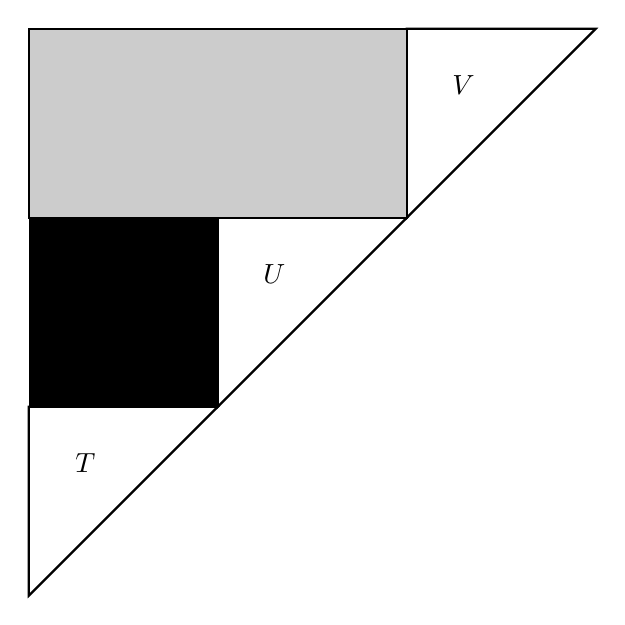
\begin{tikzpicture}[scale=1.2]

% T triangle
\draw[thick]
(0,0) -- (0,2) -- (2,2) -- cycle;
\node at (0.6,1.4) {$T$};

% U triangle
\draw[thick]
(2,2) -- (2,4) -- (4,4) -- cycle;
\node at (2.6,3.4) {$U$};

% V triangle
\draw[thick]
(4,4) -- (4,6) -- (6,6) -- cycle;
\node at (4.6,5.4) {$V$};

% black square between T and U
\fill[black] (0,2) rectangle (2,4);

% gray completed rectangle between U and V
\fill[gray!40] (0,4) rectangle (4,6);

% outline gray rectangle
\draw[thick] (0,4) rectangle (4,6);

\end{tikzpicture}
\]
\end{proof}

\end{document}